\documentclass[a4paper]{article}

\usepackage{color}
\usepackage{url}
\usepackage[T2A]{fontenc} % enable Cyrillic fonts
\usepackage[utf8]{inputenc} % make weird characters work
\usepackage{graphicx}

\usepackage[english,serbian]{babel}
%\usepackage[english,serbianc]{babel} %ukljuciti babel sa ovim opcijama, umesto gornjim, ukoliko se koristi cirilica

\usepackage[unicode]{hyperref}
\hypersetup{colorlinks,citecolor=green,filecolor=green,linkcolor=blue,urlcolor=blue}

%\newtheorem{primer}{Пример}[section] %ćirilični primer
\newtheorem{primer}{Primer}[section]

\begin{document}

\title{Stiven Hoking\\ \small{Seminarski rad u okviru kursa\\Tehničko i naučno pisanje\\ Matematički fakultet}}

\author{Lazar Rajčić\\ lazarrajcic23@gmail.com}
\date{14.~novembar 2022.}
\maketitle

\abstract{
Razlog zašto smo izabrali da pišemo o Stivenu Hoking-u jeste da bi ljudima približili njegove doprinose nauci uprkos barijerama koje je predstavljala njegova bolest. Unutar ovog seminarskog smo ispričali kratko njegovu životnu priču i objasnili neke od njegovih teorija.  

\tableofcontents

\newpage

\section{Uvod}
\label{sec:uvod}
Pre nego sto počnemo sa pričom o životu Stivena Hokinga i njegovim dostignućima moramo napraviti mali uvod u to ko je zapravo Stiven Hoking.
Stiven Hoking je bio engleski teoretski fizičar i kozmolog. Zbog njegovih doprinosa fizici smatran je za jednog od najvecih naučnika svog vremena. Njegovi doprinosi fizici se uglavnom nalaze u domenu našeg poznavanja crnih rupa ali o tome ćemo detaljnije pisati u zaglavlju Karijera. Zbog ovoga smatramo da je jako važno približiti njegova dostignuća ljudima.
Tematika ovog seminarskog rada je život i dostignuća Stivena Hokinga. Manja zaglavlja seminarskog su: Život, koji se dalje deli na život pre i posle dijagnoze, i Karijera.

\section{Život}
\subsection{Život pre dijagnoze i dijagnoza (rani život)}
Hoking se rodio 8. Januara 1942. Godine, tačno na tristotu godišnjicu smrti njegove velike inspiracije Galilea Galileja. Iako iznenđujuće nije bio najbolji ucenik, Stivena je od ranih nogu izuzetno interesovalo kako univerzum funkcioniše. Čak će u kasnijim godinama reći da ako razumemo kako univerzum radi mozemo u neku ruku i da ga kontrolišemo. Ova znatiželja koja će ga kasnije u životu gurati u napredovanju kariere, u školi mu je zaslužila nadimak Ajnštajn. Planovi za dalje studiranje matematike ometeni su od strane njegovog oca koji je smatrao da u tome nema budućnosti. Usledio je kompromis, kojim je odlučeno da će Stiven da pohađa osnovne studije na polju fizike na Oksfordu. Osnovne studije je zavrsio 1962. godine sa diplomom prvog reda posle čega se uputio na dalje obrazovanje na Kembridž univerzitetu.


\begin{figure}[h!]
\centering
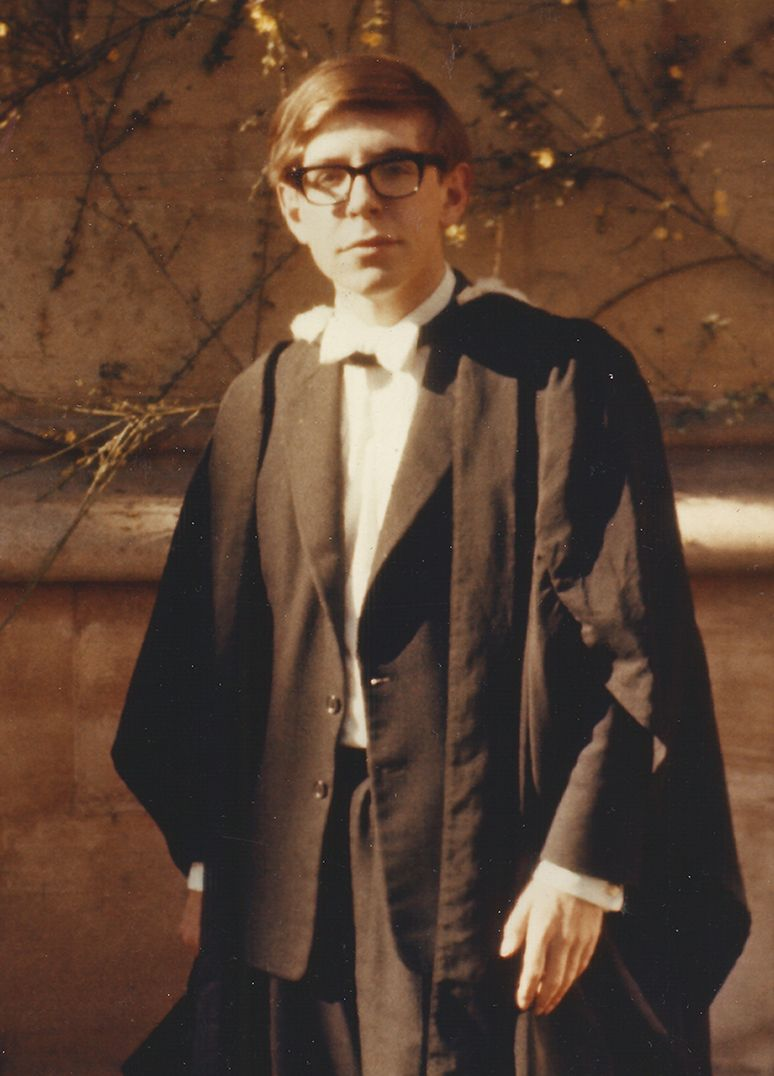
\includegraphics[width=0.5\textwidth]{Hoking,PreDijagnoze.jpg}
\caption{Hoking, na dodeli diploma 1960.}
\end{figure}



\end{document}
